\section{Functional Role of Remixing}

I analyze the role remixing plays in participating in an online community of creators.
I look at how several forms of remixing (Figure~\ref{fig:function} are represented in the Scratch Online Community, how their use evolves, and how they do or do not support sociability and creative practices.
I analyze people's remixing behavior including their: 
1) modifying existing work, 
2) reusing components, 
3) collaborating with others in groups, 
4) persuading crowds to join remixing chains, 
5) inspiring others with ideas for new creations or 
6) self-appropriating their work to create something. 

\begin{figure}
\centering
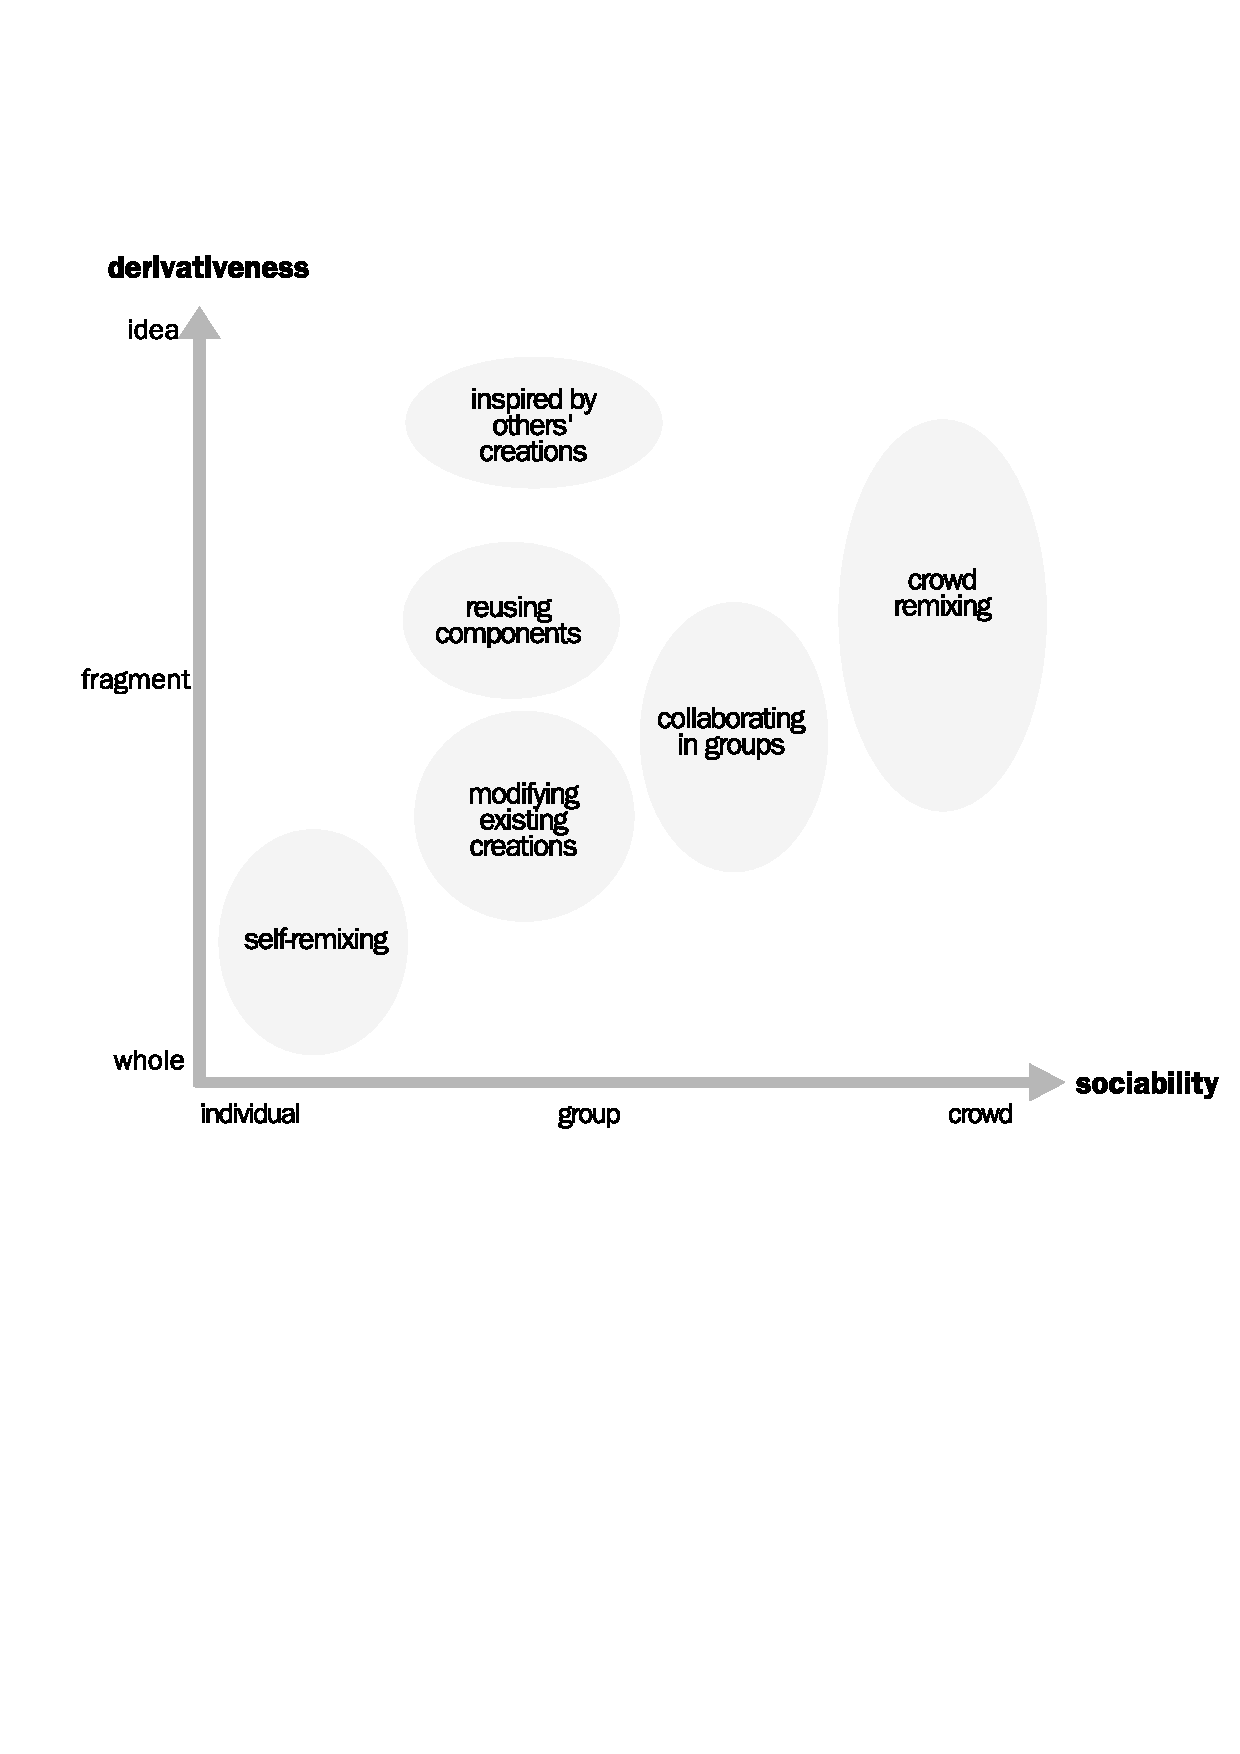
\includegraphics[width=3.25in]{figures/function.pdf}
\caption{Functional roles of remixing in the social and produc-focus dimensions}
\label{fig:function}
\end{figure}

% TODO:
% Proposed work:
% - Evolution of each type.
% - How do they engage in these different forms of production.
% - To what extent do these different forms of remixing support:
% a) scaffolding,  b) committment, c) creative and d) collaborative practices? e) reputation
% 	Look at people who get started by remixing and compare it to those who don't. Follow take other pats.
% 1. Modifying existing work. 
% 4. Crowds: coloring contests
% Some of these roles are analyzed from a network perspective. For example, the network of people engaged in colloring contests represents a group of people involved in a gift exchange network.
